\subsection{Fachmodell}
Das Fachmodell wurde in die vier Klassendiagramme Produkt (Abbildung \ref{fig:dm-product}), Design (Abbildung \ref{fig:dm-design}), Entwurf (Abbildung \ref{fig:dm-entwurf}) und Bühne (Abbildung \ref{fig:dm-editor}) unterteilt. Die Sichten beziehen sich ausschließlich auf die fachliche Relevanz für den FreeDesign-Editor und auf dessen Kernaufgaben. Dies gilt im besonderen für die Sicht des Produkts, da für dieses im umgebenden System weitere fachliche Fakten relevant sind. 
Für alle Assoziationen in den folgenden Klassendiagrammen gilt, wenn keine Multiplizität angegeben wurde, gilt der Wert Eins. 

\begin{figure}[H]
    \centering
    \caption{Die fachliche Sicht des Produkts bezogen auf den FreeDesign-Editor.}
    \label{fig:dm-product}
    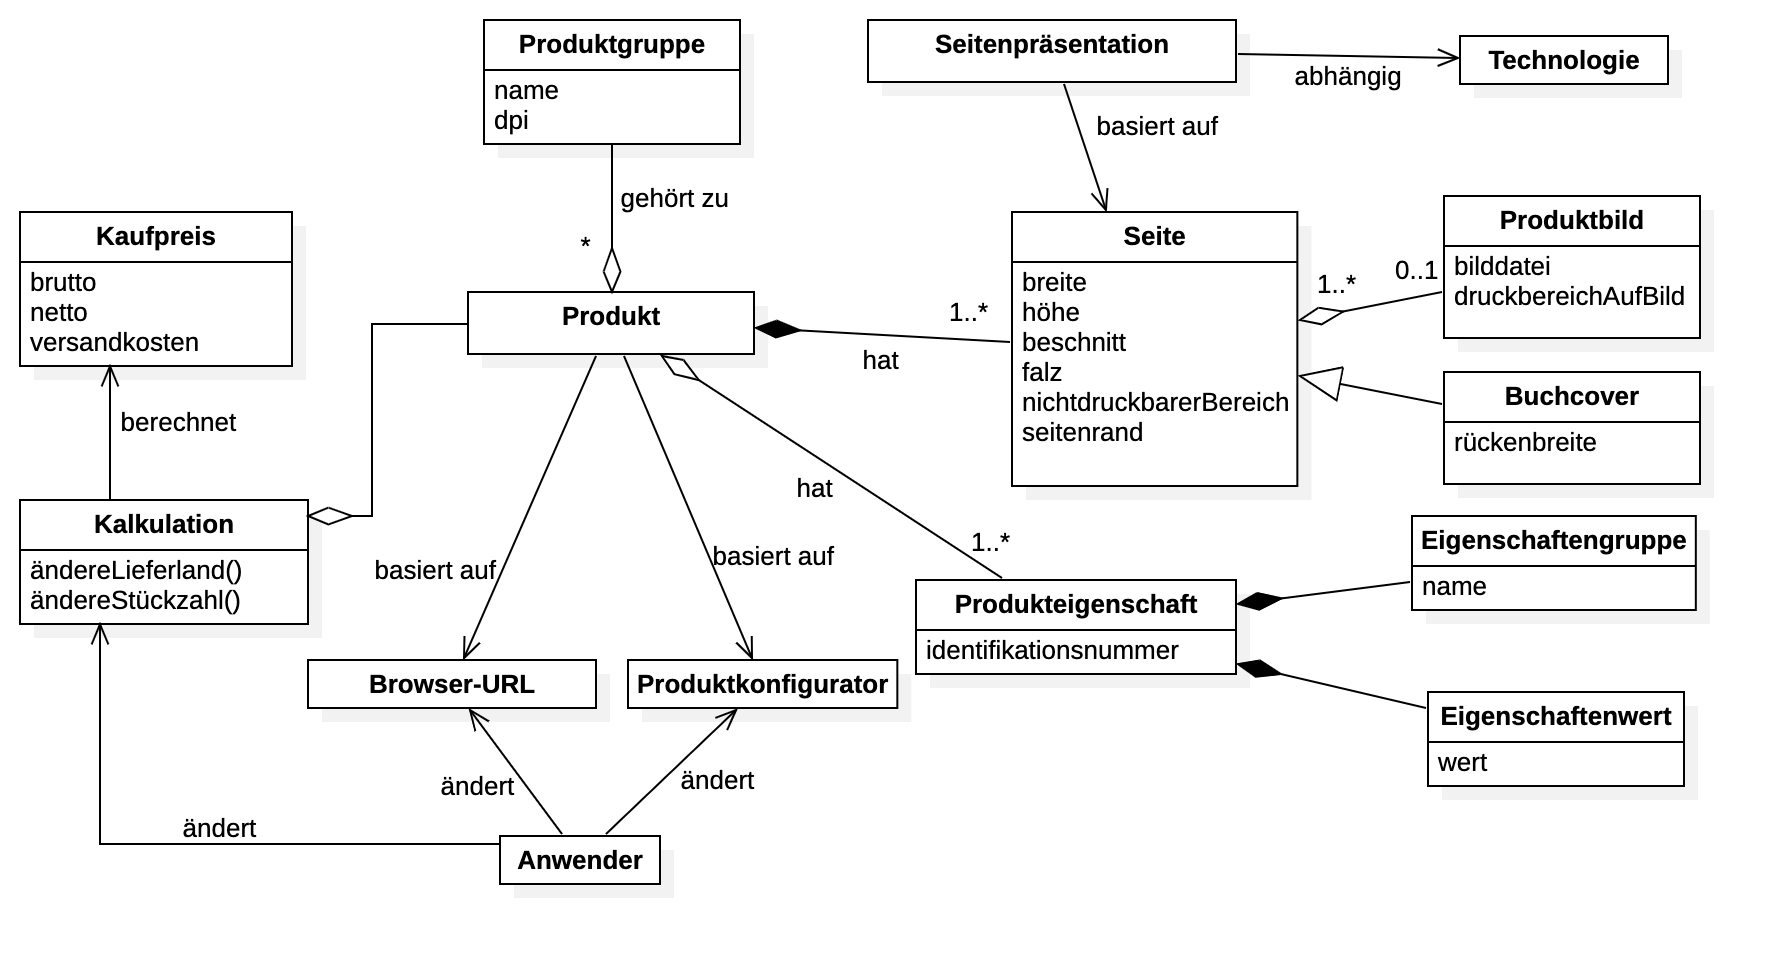
\includegraphics[width=1\textwidth]{diagrams/Soll-Architektur/DM-Produktstruktur.png}
\end{figure}

Jedes Produkt gehört einer Produktgruppe an und hat mehrere Eigenschaften. Jede Eigenschaft gehört einer Eigenschaftengruppe an und besitzt einen Wert. Ein Produkt darf nicht mehrfach Eigenschaft der selben Eigenschaftengruppe besitzten. Die Tabelle \ref{table:BspProdukt} enthält einen Beispieldatensatz für ein Produkt der Gruppe Visitenkarte.
\begin{table}[H]
    \centering
    \caption{Beispieldatensatz für ein doppelseitige Visitenkarte (gekürzt)}
    \label{table:BspProdukt}
    \begin{tabular}{c|c|c}
        \multicolumn{3}{l}{\textbf{Produktgruppe:} Visitenkarte}  \\
        \textbf{Identifikationsnummer} & \textbf{Gruppennamen} & \textbf{Wert} \\
        8456 & Seitenzahl & 2-seitig \\
        6543 & Format & 80,0 mm x 50,0 mm \\
        4561 & Papier & 350 g/m$^2$ \\
    \end{tabular}
\end{table}

Für den FreeDesign-Editor sind die Produkteigenschaften jedoch nur für die Kommunikation mit API relevant. Dem Editor muss beim Öffnen als Minimalwert der Name der Produktgruppe als URL-Parameter übergeben werden. Es kann jedoch auch einen Teilmenge der Identifikationsnummern für Produkteigenschaften in URL mitgeben werden. Für die fehlenden Eigenschaft werden Standardwerte, die auf dem Server hinterlegt sind genutzt. Der Anwender hat weiterhin die Möglichkeit über einen Produktkonfigurator das Produkt zu ändern.
Die Darstellung des Produktes im FreeDesign-Editor wird bei Einführung durch die Fachabteilung festgelegt. Dabei wird jede Seite beschrieben, wobei die Beschreibungen sehr Produktspezifisch sind. In Abbildung \ref{fig:dm-product} wurden die üblichen Seiteneigenschaften hinterlegt. Einige Produkt, wie Text- und Werbeprodukte, werden für in die Darstellung mit im FreeDesign-Editor mit einem Produktbild hinterlegt. Auf Basis der Seiteneigenschaften wird eine Präsentation der Seite erzeugt, welche von der verwendeten Technologie abhängt. 

\begin{figure}[H]
    \centering
    \caption{Die fachliche Sicht eines Designs.}
    \label{fig:dm-design}
    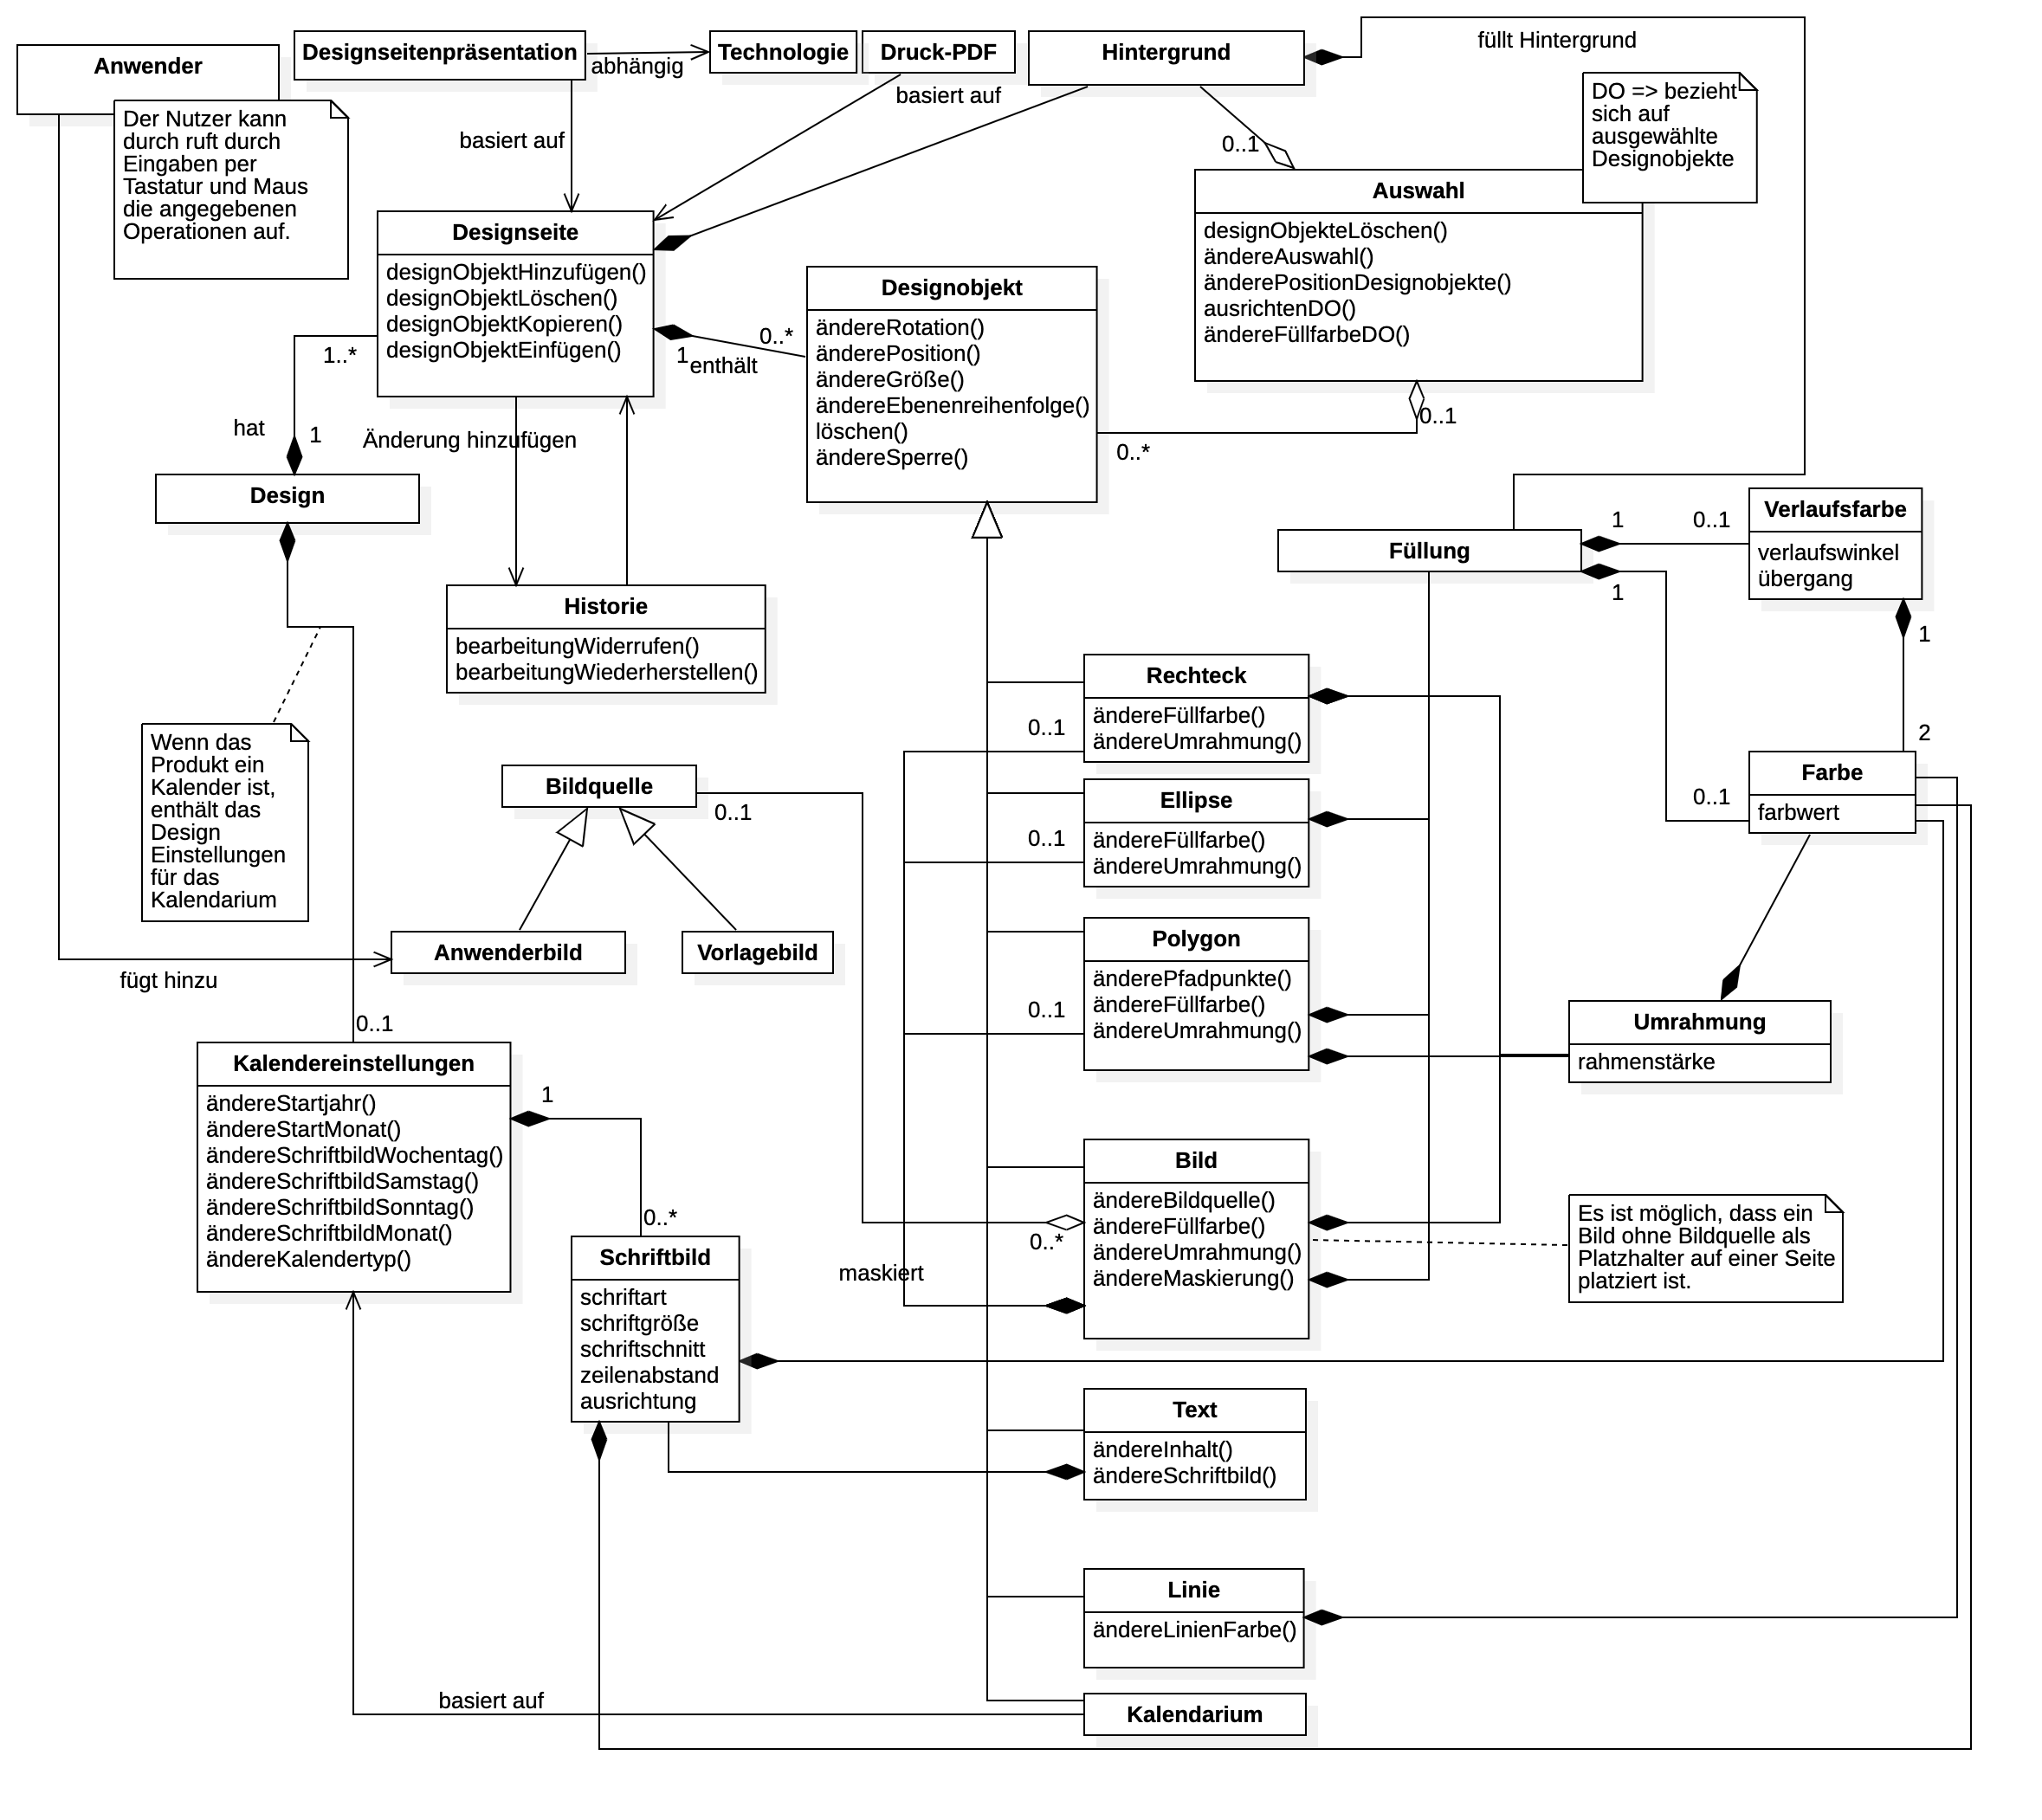
\includegraphics[width=1\textwidth]{diagrams/Soll-Architektur/DM-Designstruktur.png}
\end{figure}

Ein Design besteht aus mindestens einer Designseite. Diese wiederum enthält einen Hintergrund und einer Menge von grafischen Elementen, welche als Designobjekte bezeichnet werden. Die Designobjekte bieten dem Anwender Operationen zum Verändern der Objekte. Jede Änderung wird in einer Historie, welche sich auf die Designseite der Änderung bezieht, festgehalten. Änderungen können über die Historie vom Anwender Widerrufen und Wiedergestellt werden.

Der Anwender hat die Möglichkeit eigene Bilder im Design zu verwendet. Ein Bild kann aber auch von einer Designvorlage stammen. 

Für das Bearbeiten von Designobjekten muss eine Auswahl durch den Anwender getroffen werden. 

Kalender-Produkten stellen einen Spezialfall für das Design dar, da für sie automatisiert Kalendarien in die Designseiten generiert werden.  Dem Anwender wird die Möglichkeit gebot das Aussehen des Kalendariums zu beeinflussen, sowie das Startjahr sowie den Startmonat festzulegen.

Auf der Basis der Designseite wird eine PDF für den Druck des Produktes erstellt, sowie Präsentationen der Designseite unter Verwendung spezifischer Technologien.

\begin{figure}[H]
    \centering
    \caption{Die fachliche Sicht des Entwurfs.}
    \label{fig:dm-entwurf}
    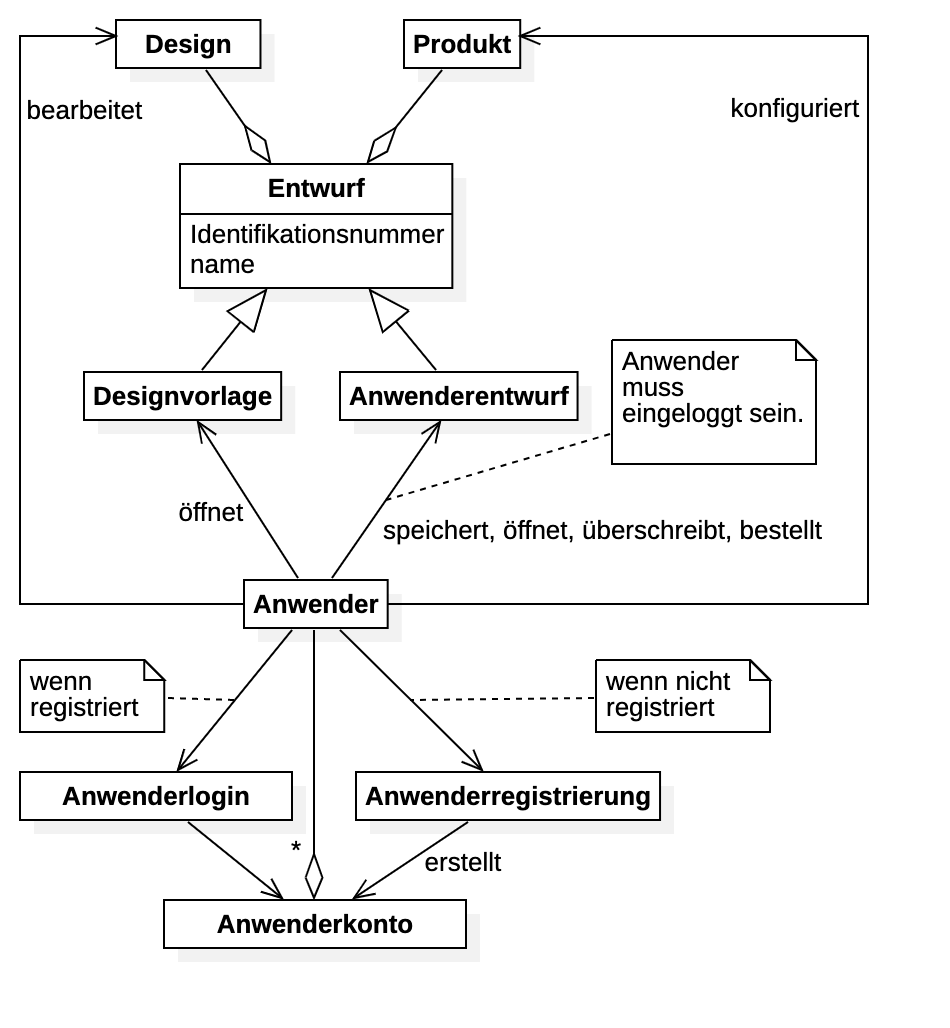
\includegraphics[width=.5\textwidth]{diagrams/Soll-Architektur/DM-Anwenderstruktur.png}
\end{figure}

Der Entwurf setzt sich aus einem Design und einem Produkt zusammen und kann vom Anwender zur späteren Bearbeitung gespeichert werden. Jeder Bestellposition ist ebenefall genau ein Entwurf zugeordnet. Für das Speichern und Bestellen eines Entwurfs muss der Anwender ein Anwenderkonto besitzten und in dieses eingeloggt sein.

\begin{figure}[H]
    \centering
    \caption{Die fachliche Sicht der Bühne.}
    \label{fig:dm-editor}
    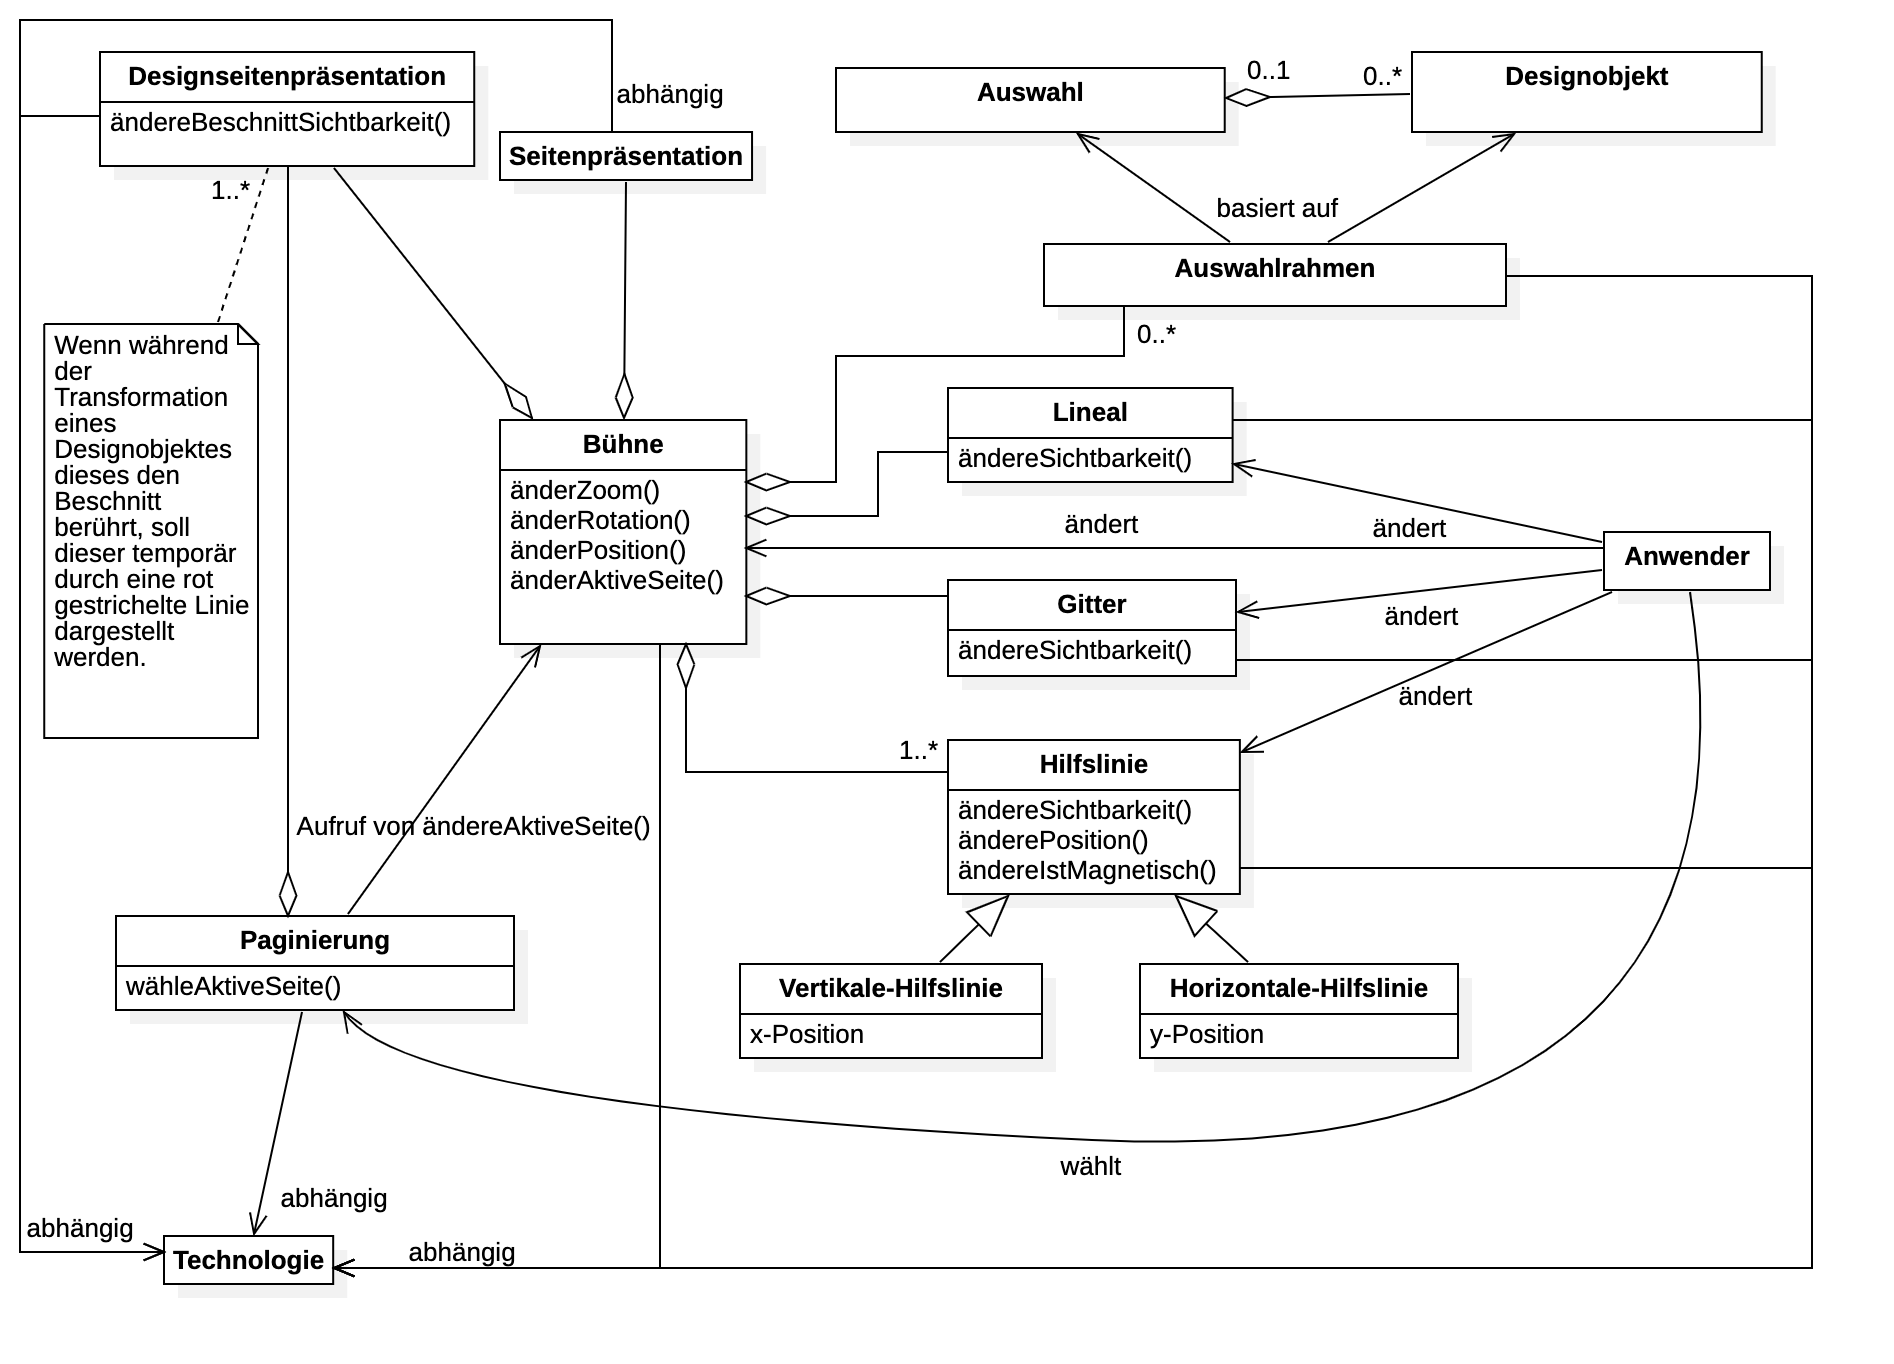
\includegraphics[width=1\textwidth]{diagrams/Soll-Architektur/DM-Editor.png}
\end{figure}
Auf der Bühnen wird eine Produktseite mit der zugehörigen Produktseite präsentiert, was als die aktive Produktseite bezeichnet wird. Über eine Paginierung kann die aktive Seite gewechselt werden. Die Bühne integriert weiterhin Werkzeug, die das Bearbeiten des Designs unterstützen. 